\documentclass[tikz,border=2pt]{standalone}
\usepackage{amsmath,amssymb}
\usepackage{pgfplots}
\pgfplotsset{compat=1.18}

\begin{document}
% X = 1 or 3 with probability 1/2, Y | X ~ Pois(X). Condition on X: each case has an easy mean
% and variance; Var(Y) = E[Var(Y|X)] + Var(E[Y|X]) = 2 + 1 = 3.
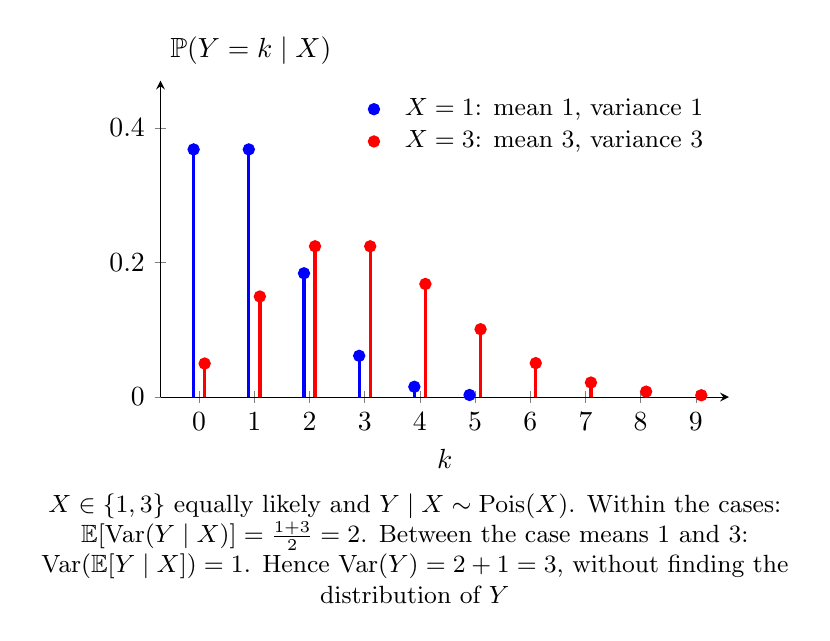
\begin{tikzpicture}
	\begin{axis}[
		axis lines=left, xmin=-0.7, xmax=9.6, ymin=0, ymax=0.47,
		xtick={0,1,...,9}, ytick={0,0.2,0.4},
		xlabel={$k$}, ylabel={$\mathbb{P}(Y=k\mid X)$}, ylabel style={rotate=-90, anchor=south west, at={(axis description cs:0,1.02)}},
		width=8.8cm, height=5.6cm, clip=false,
		legend style={draw=none, fill=none, font=\small, at={(0.98,0.98)}, anchor=north east}, legend cell align=left
		]
		\addplot[ycomb, blue, very thick, mark=*, mark size=1.6pt] coordinates {(-0.1,0.3679) (0.9,0.3679) (1.9,0.1839) (2.9,0.0613) (3.9,0.0153) (4.9,0.0031)};
		\addlegendentry{$X=1$: mean $1$, variance $1$}
		\addplot[ycomb, red, very thick, mark=*, mark size=1.6pt] coordinates {(0.1,0.0498) (1.1,0.1494) (2.1,0.2240) (3.1,0.2240) (4.1,0.1680) (5.1,0.1008) (6.1,0.0504) (7.1,0.0216) (8.1,0.0081) (9.1,0.0027)};
		\addlegendentry{$X=3$: mean $3$, variance $3$}
	\end{axis}
	\node[anchor=north, font=\small, align=flush center, text width=9.6cm] at ([yshift=-2pt]current axis.outer south) {$X\in\{1,3\}$ equally likely and $Y\mid X\sim\operatorname{Pois}(X)$. Within the cases: $\mathbb{E}[\operatorname{Var}(Y\mid X)]=\tfrac{1+3}2=2$. Between the case means $1$ and $3$: $\operatorname{Var}(\mathbb{E}[Y\mid X])=1$. Hence $\operatorname{Var}(Y)=2+1=3$, without finding the distribution of $Y$};
\end{tikzpicture}
\end{document}
